\section{Preliminary Results from BELLE Open Data}

Figure~\ref{fig:multPID} shows the multiplicity distribution of identified particles. The dominant contribution to the total multiplicity is pions and the charged hadron multiplicity distribution $N$ is shown in Fig.~\ref{fig:multHadron} and the $N$ reach the level of 70

\begin{figure}[!htb]
\begin{center}
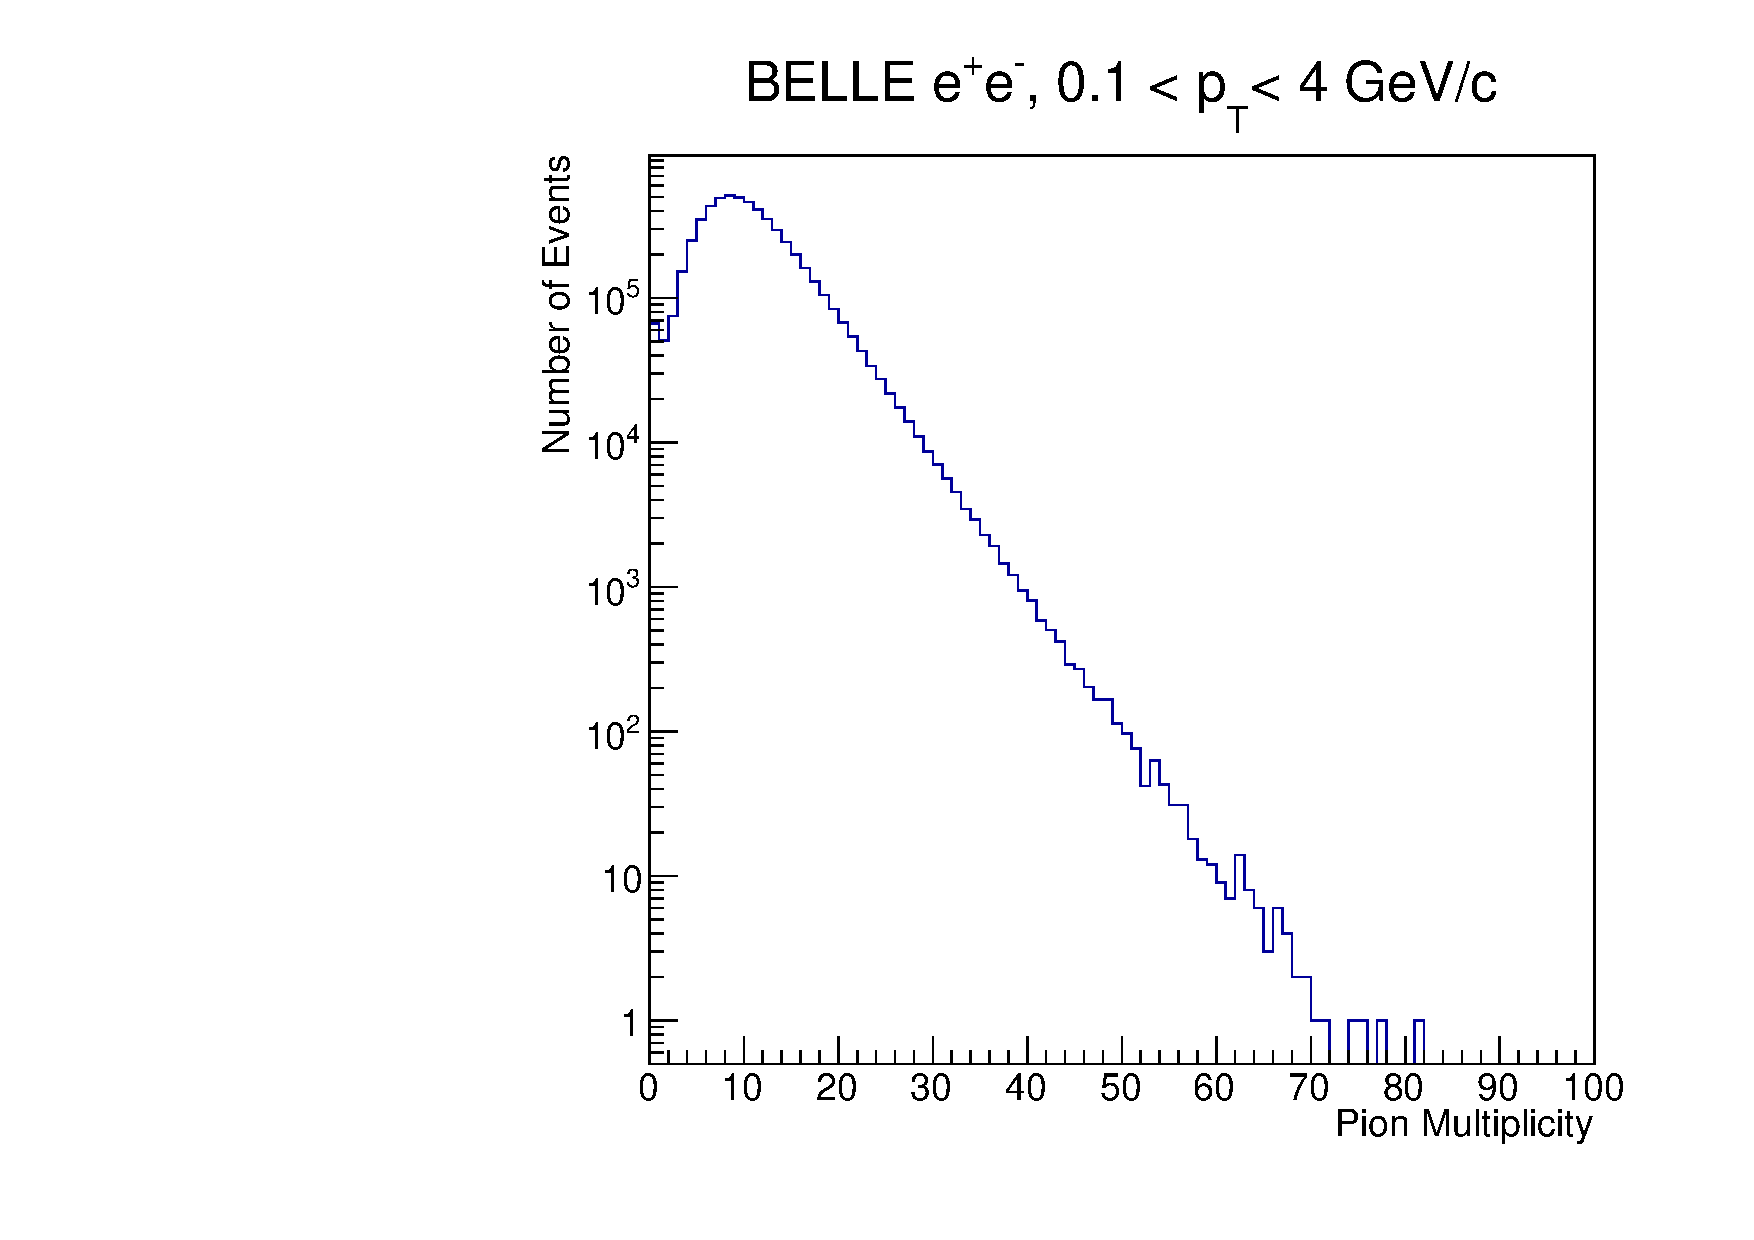
\includegraphics[width=.32\textwidth]{figures/pion_mult.pdf}
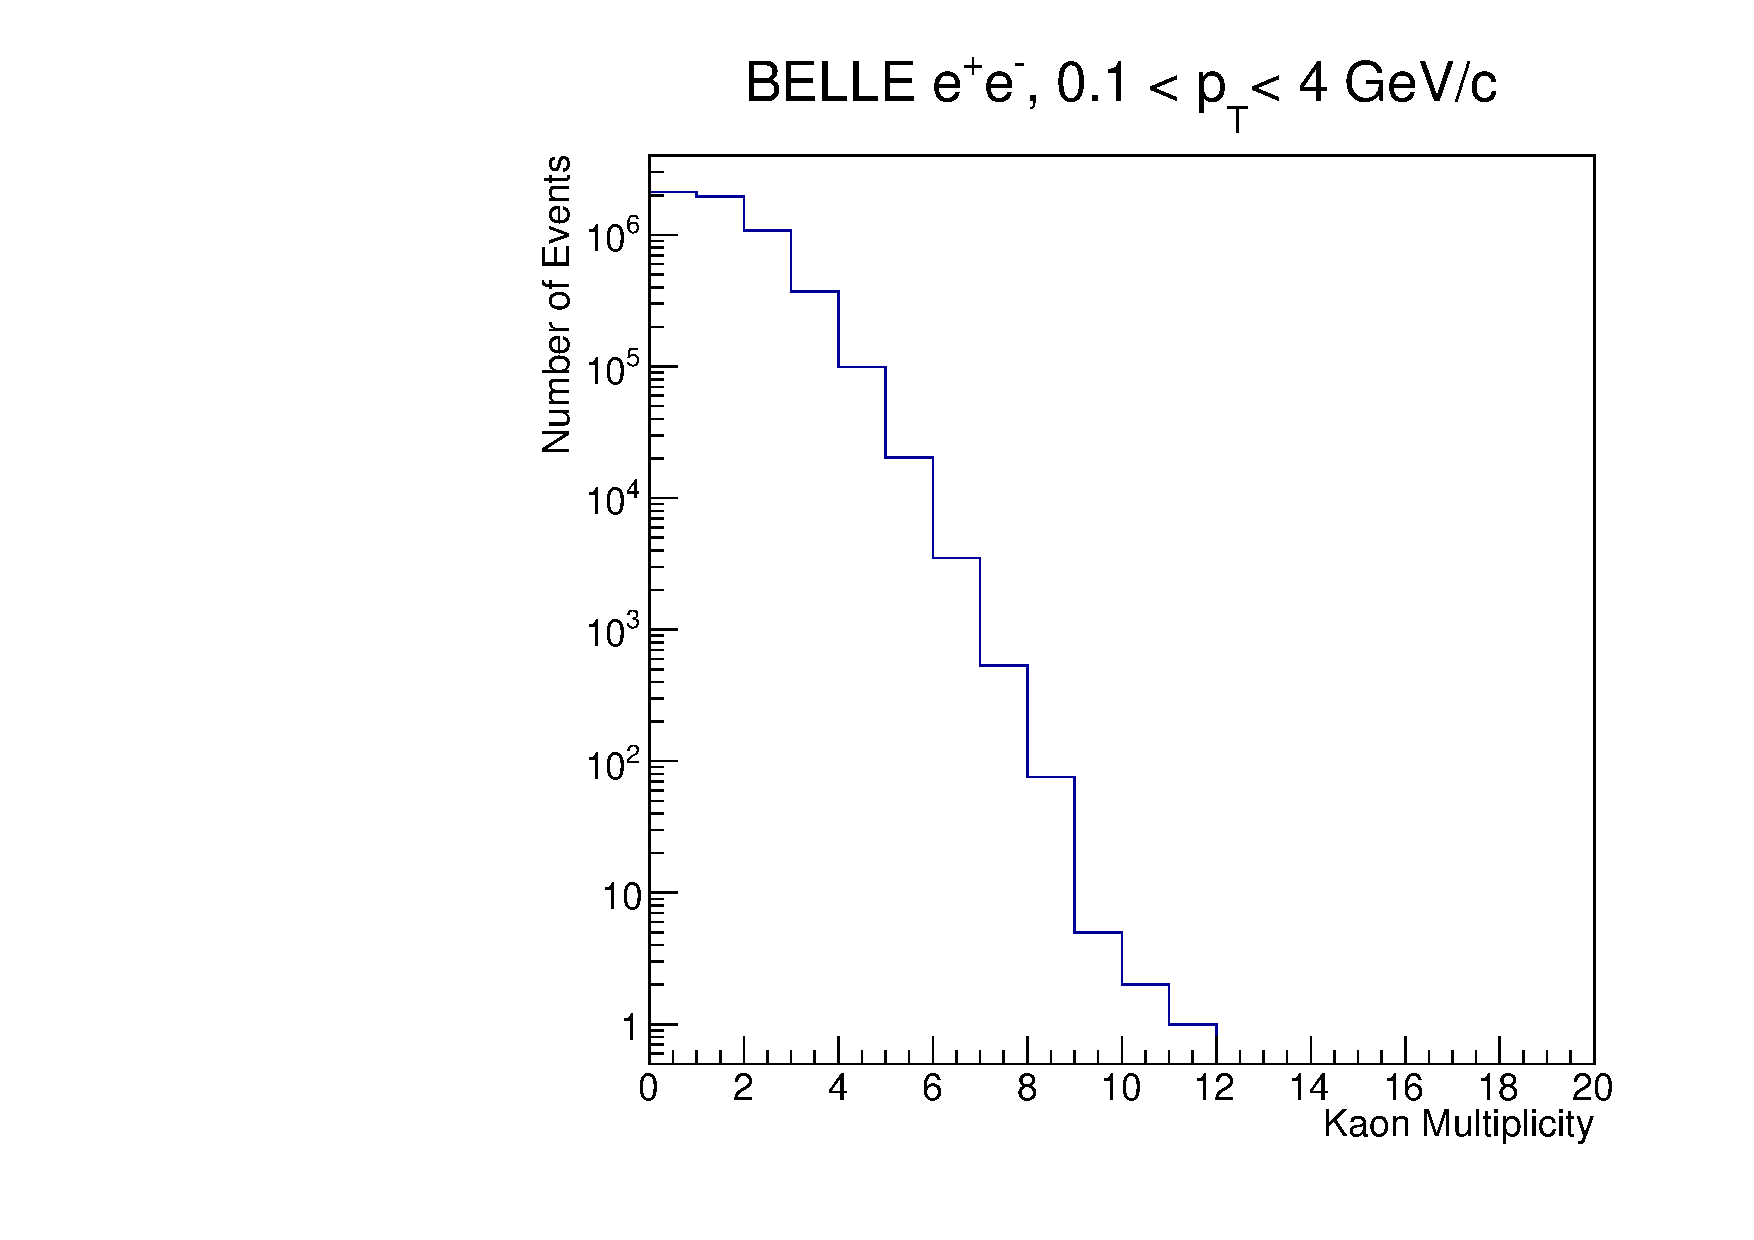
\includegraphics[width=.32\textwidth]{figures/kaon_mult.pdf}
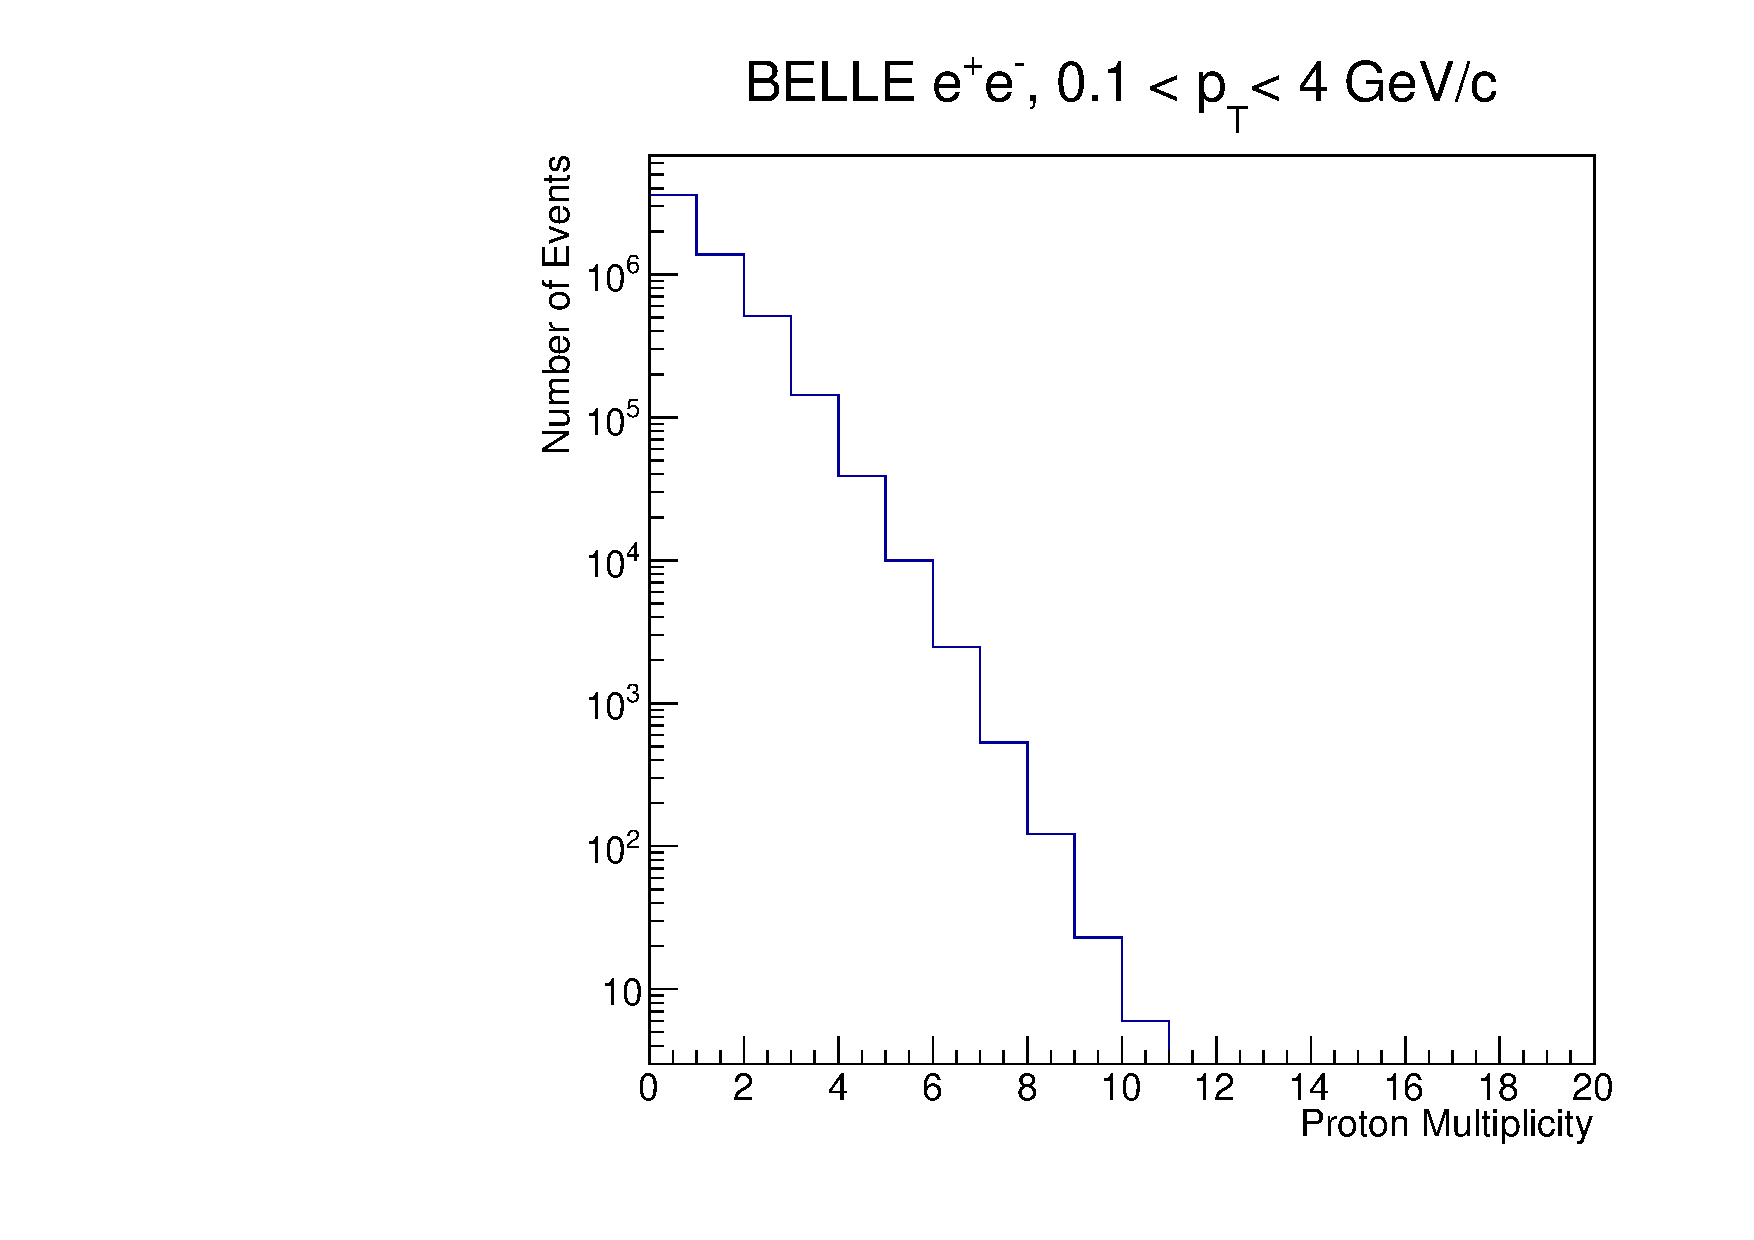
\includegraphics[width=.32\textwidth]{figures/proton_mult.pdf}
\caption{Multiplicity distributions of pions (left), kaons (middle), protons (right) }
\label{fig:multPID} 
\end{center}
\end{figure}

\begin{figure}[!htb]
\begin{center}
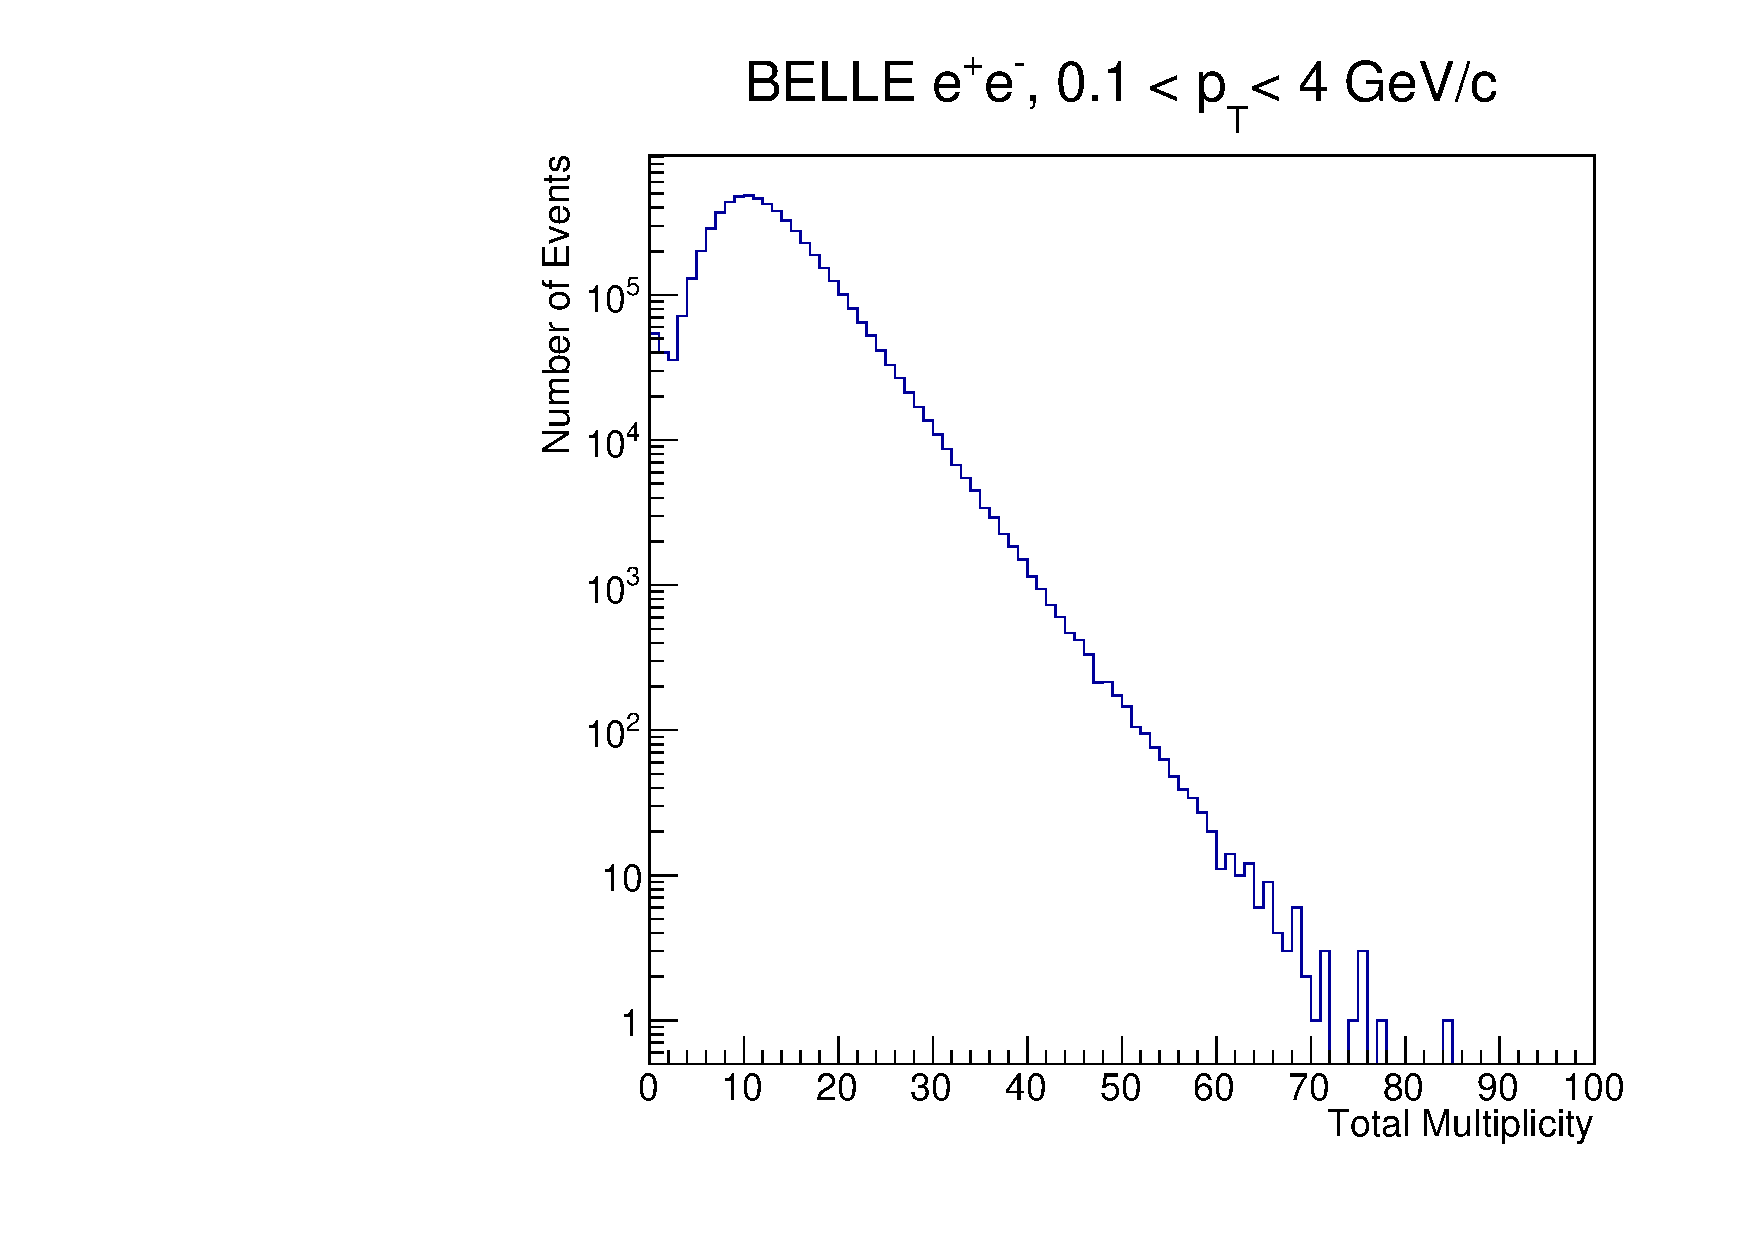
\includegraphics[width=.45\textwidth]{figures/total_mult.pdf}
\caption{Multiplicity distribution of charged hadrons (protons, kaons and pions) }
\label{fig:multHadron} 
\end{center}
\end{figure}

Two particle correlation functions are studied for the first time and the preliminary results from BELLE open data is shown in Fig.~\ref{fig:ridgeBelle}. For low-multiplicity selection $N>20$, the dominant features are the correlation peak near $(\Delta\eta,\Delta\phi)=(0,0$ for pairs of particles originating from the same jet and the elongated structure at $\Delta\phi\sim\pi$ for pairs of particles from back-to-back jets. Moving from low-multiplicity to high-multiplicity selection, the same-side jet peak and back-to-back correlation structures can be observed. However, the relative contribution of the jet peak become smaller compared to the broad structure at small $\Delta\phi$. To check if a long-range ridge structure exists, similar to that seen in high-multiplicity pp and in AA collisions over a wide range of energies, one-dimensional $\Delta\phi$ distribution over different $|\Delta\eta|$ interval are shown in Fig~\ref{fig:ProjectionMult50}. A hint of signal at $\Delta\phi=0$ could be seen in the BELLE open data, which motivates a studies with the highest statistics data taken by the BELLE collaboration.


\begin{figure}[!htb]
\begin{center}
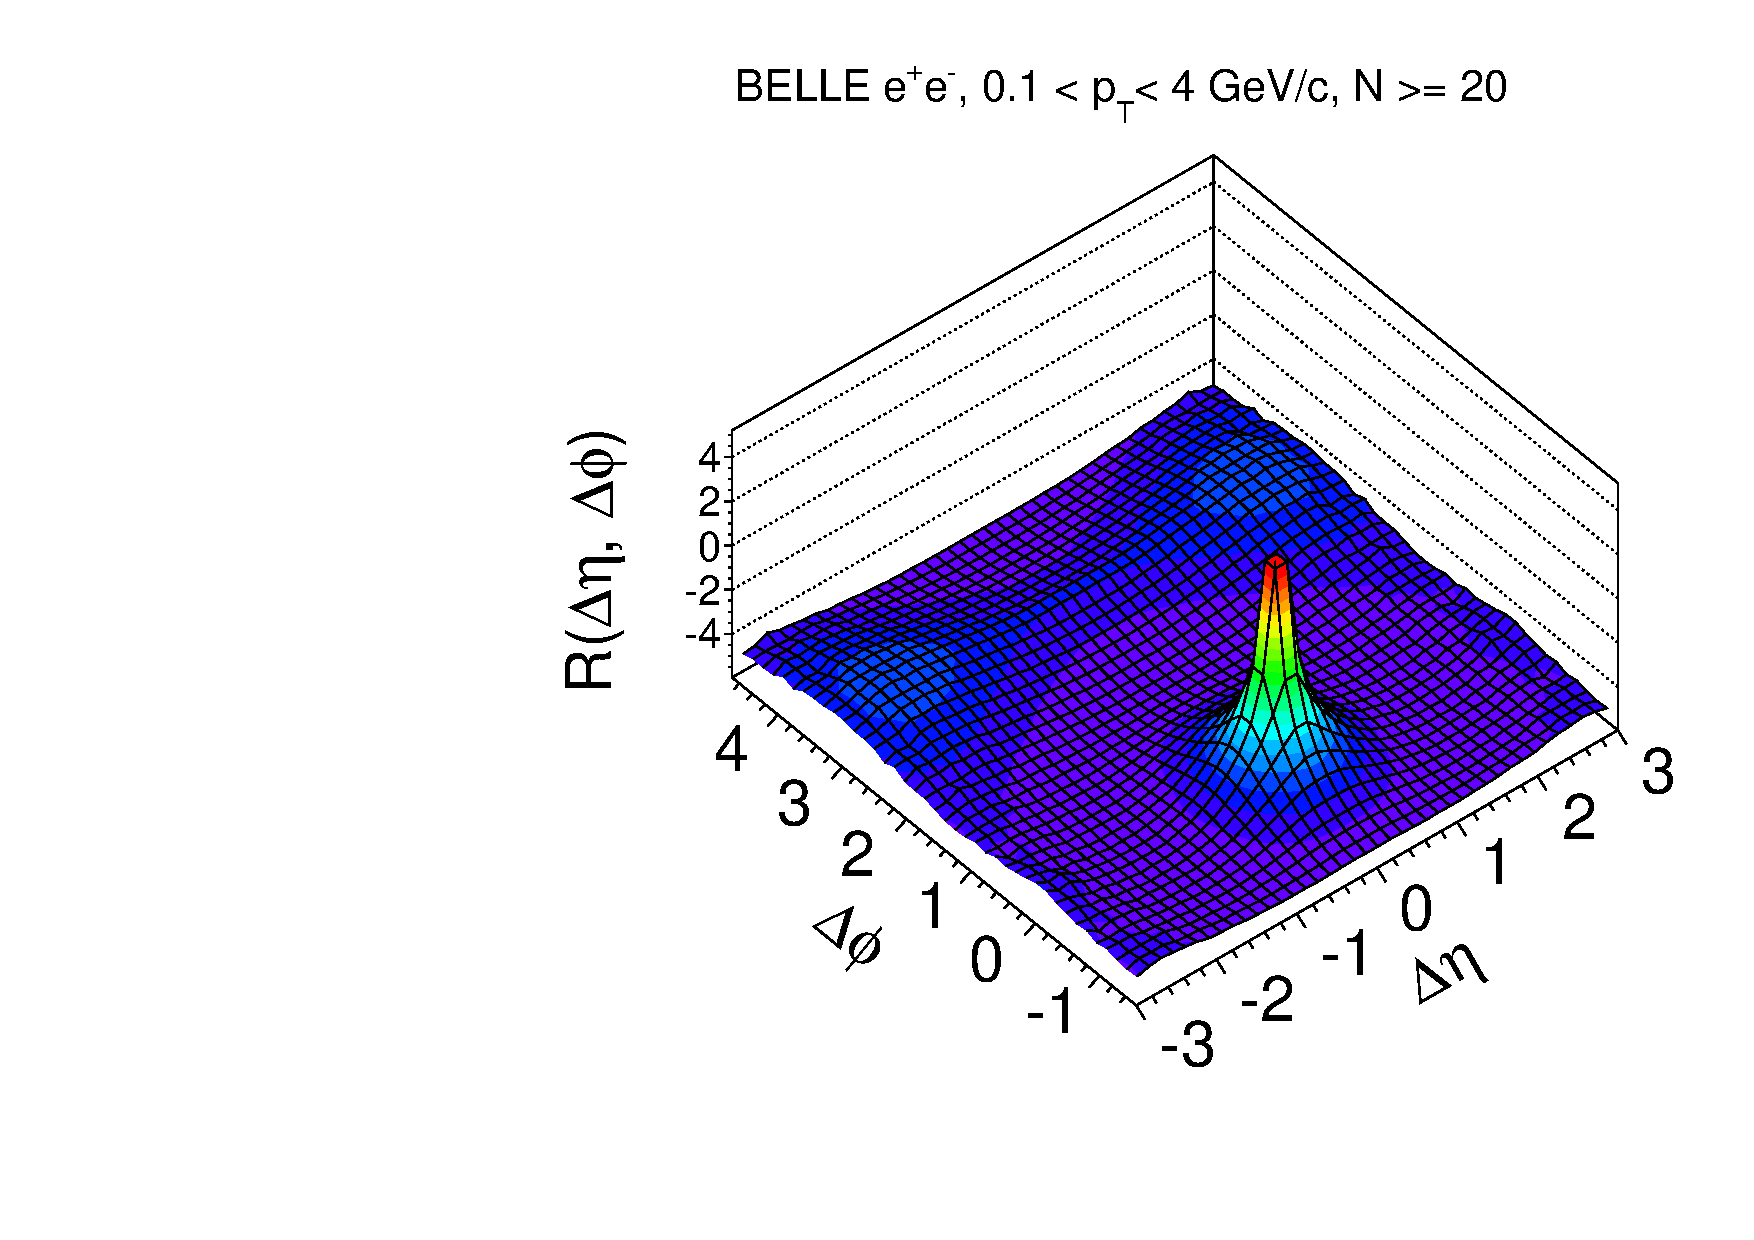
\includegraphics[width=.45\textwidth]{figures/canvasRidgeBelleMult20CutHigh0.pdf}
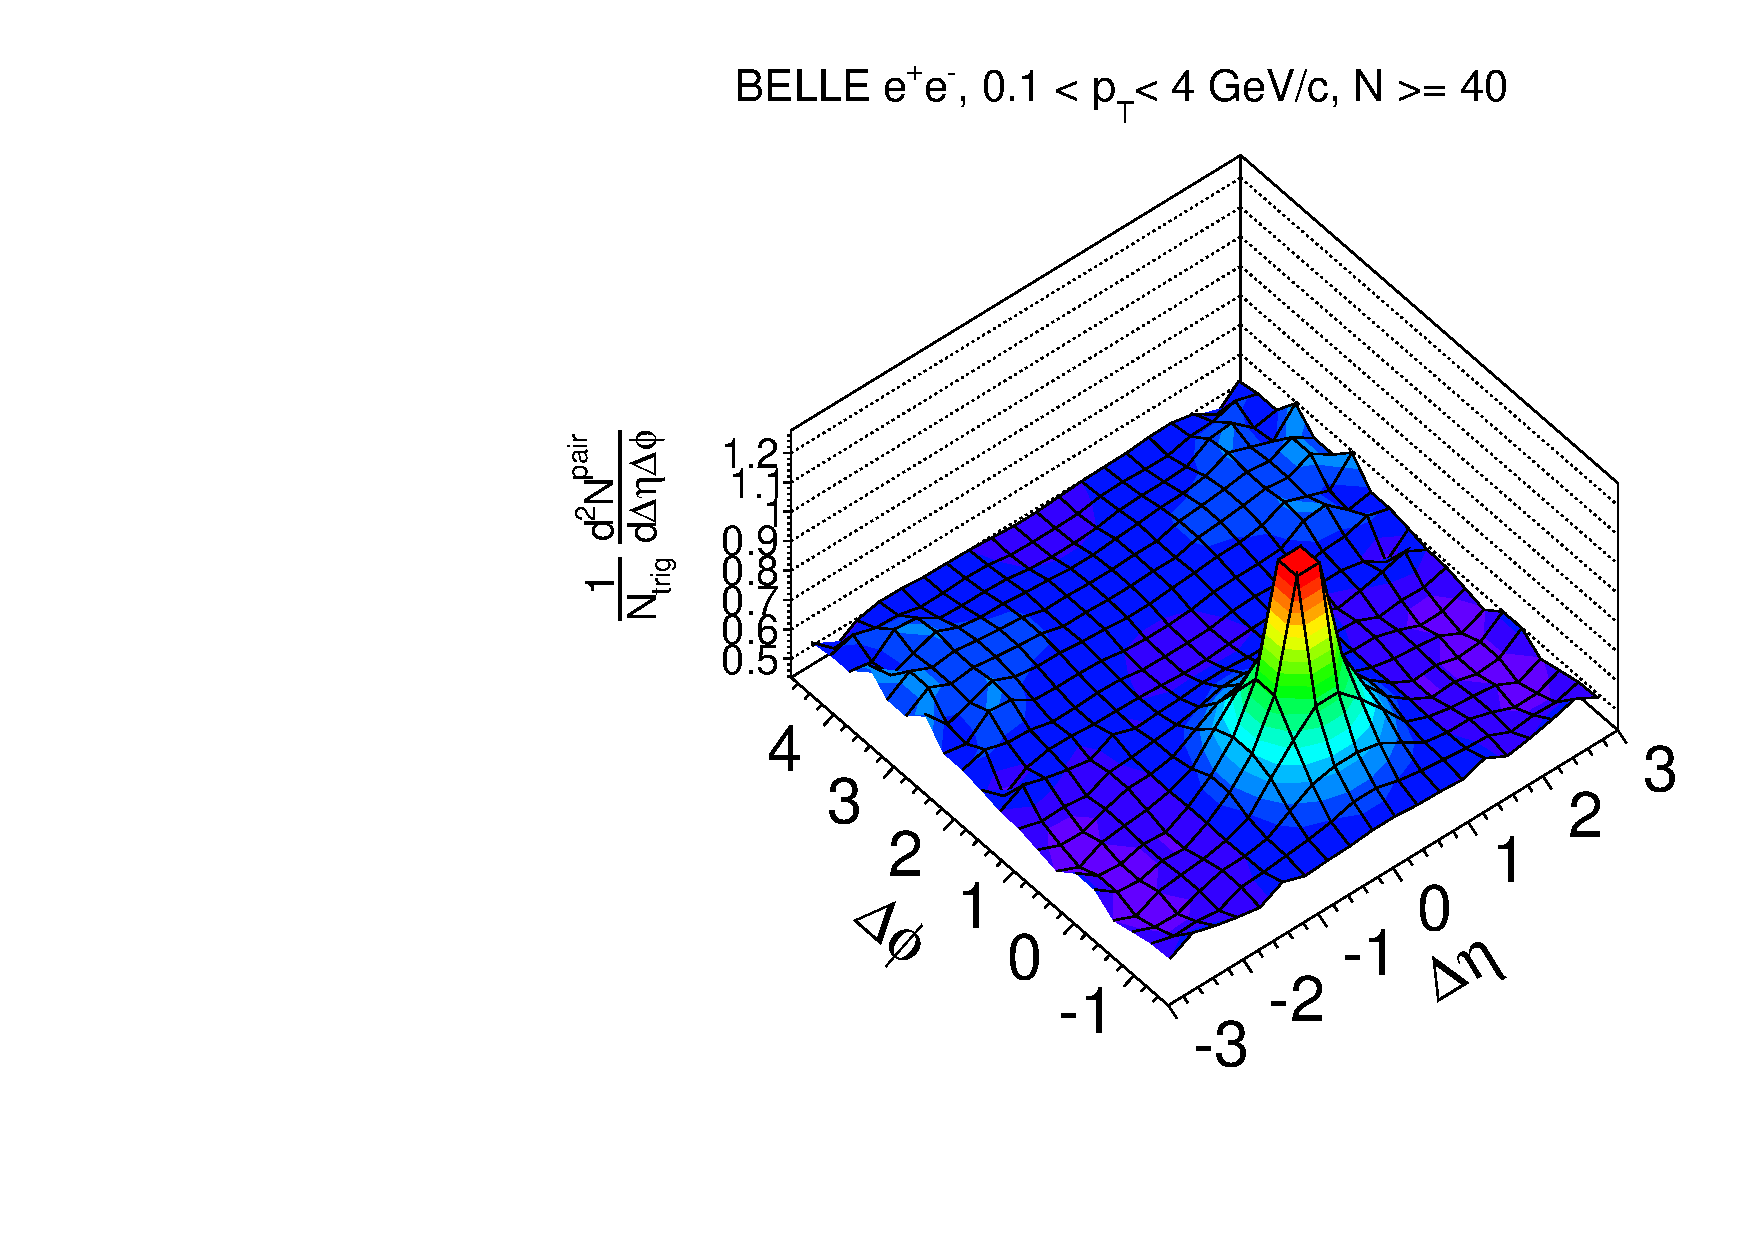
\includegraphics[width=.45\textwidth]{figures/canvasRidgeBelleMult40CutHigh0.pdf}
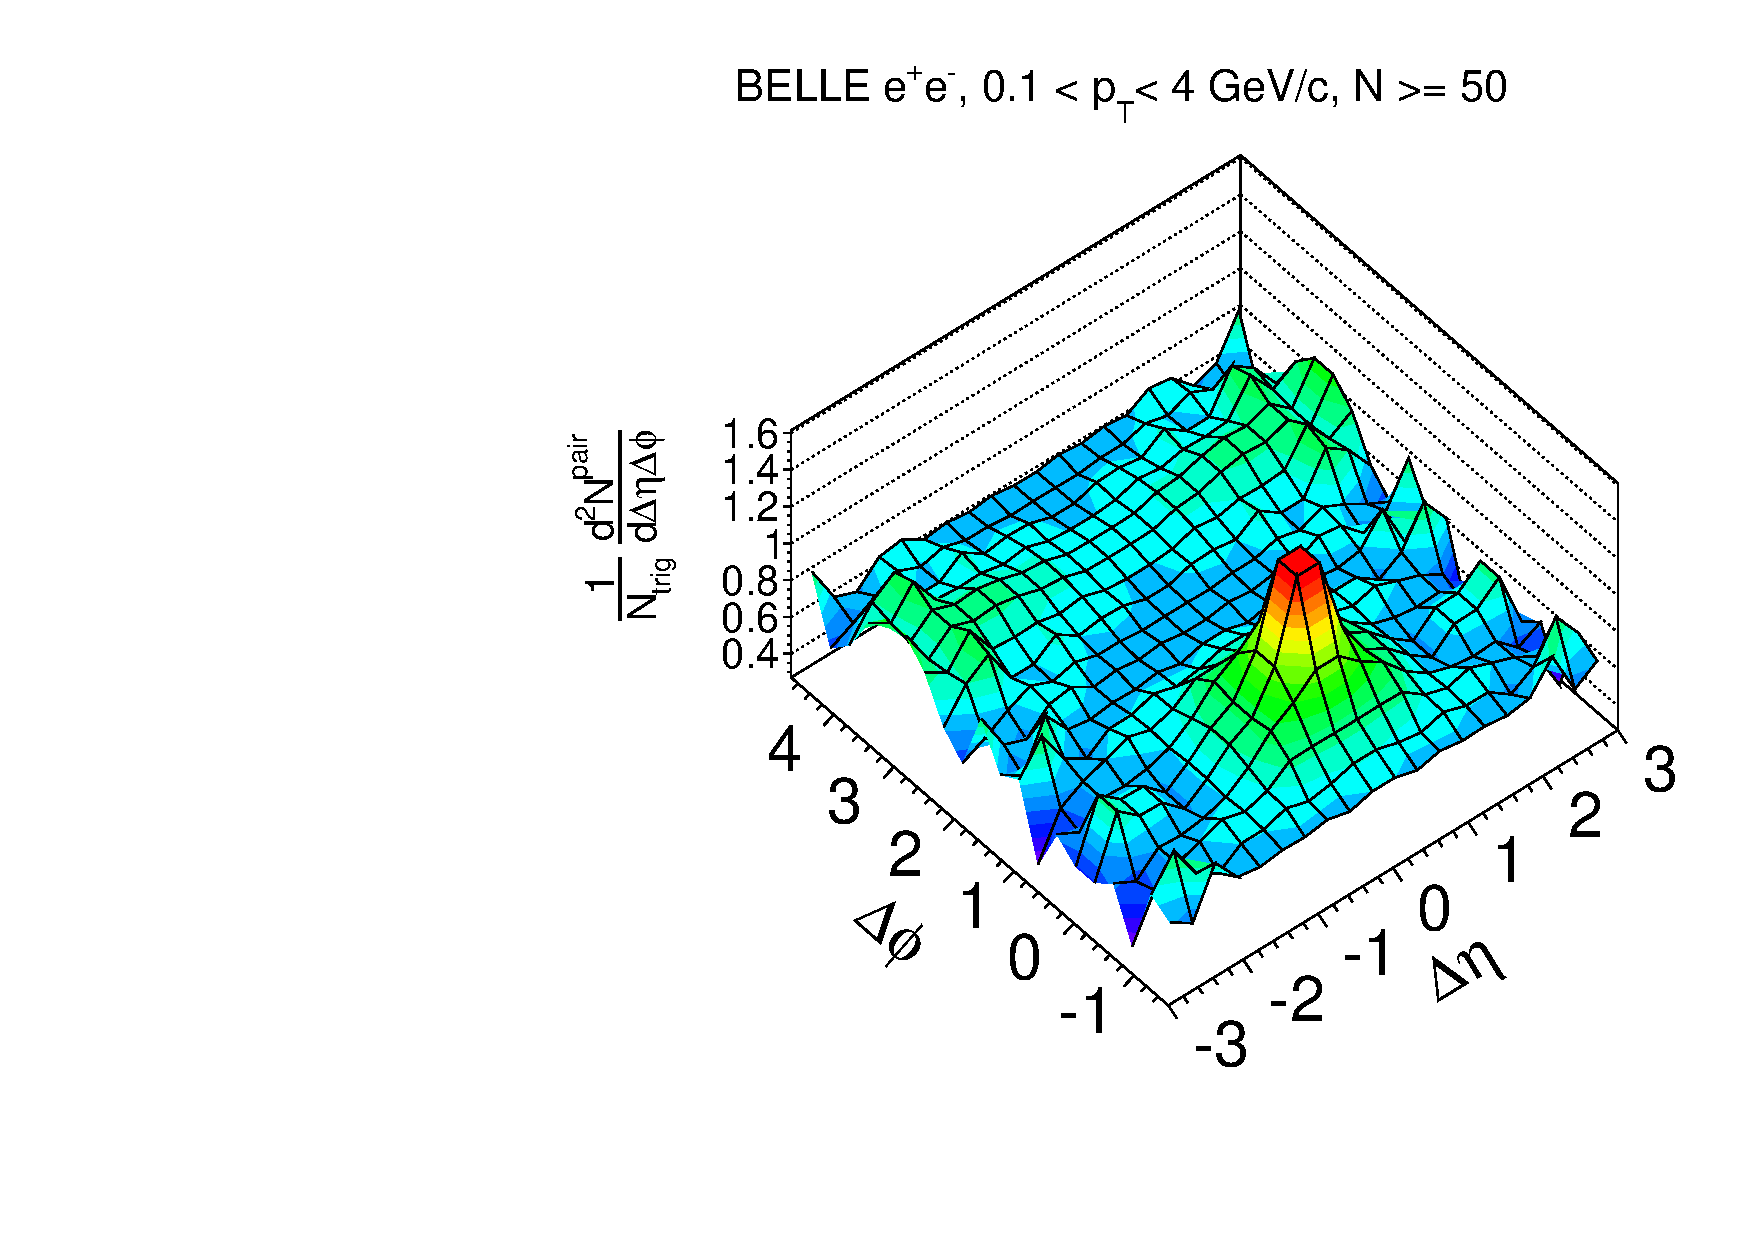
\includegraphics[width=.45\textwidth]{figures/canvasRidgeBelleMult50CutHigh0.pdf}
\caption{Two-particle correlation functions versus $\Delta\eta$ and $\Delta\phi$ in $e^{+}e^{-}$ collisions for events with particle multiplicity $>$ 20 (top left), 40 (top right), 50 (bottom).}
\label{fig:ridgeBelle} 
\end{center}
\end{figure}

\begin{figure}[!htb]
\begin{center}
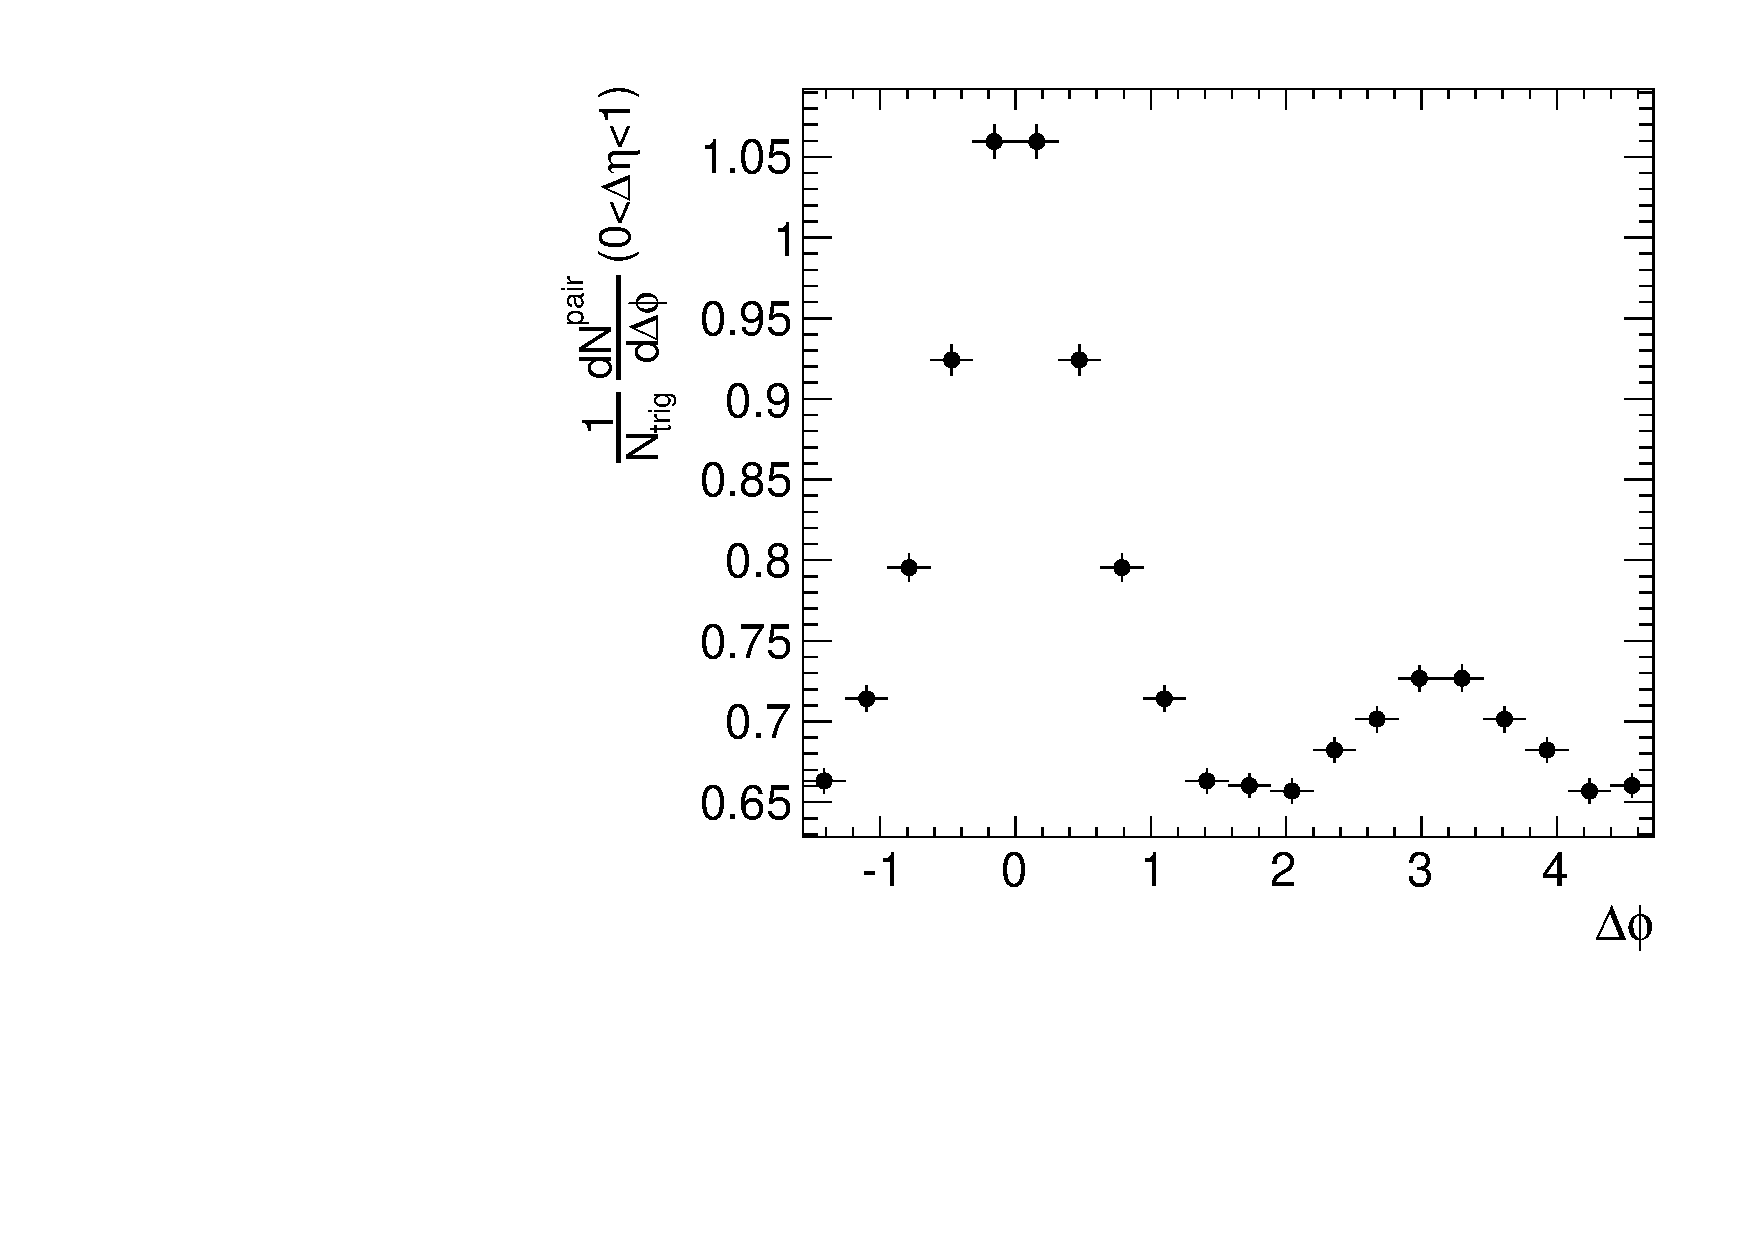
\includegraphics[width=.45\textwidth]{figures/canvasProjection_isBelle1_mult50_eta01.pdf}
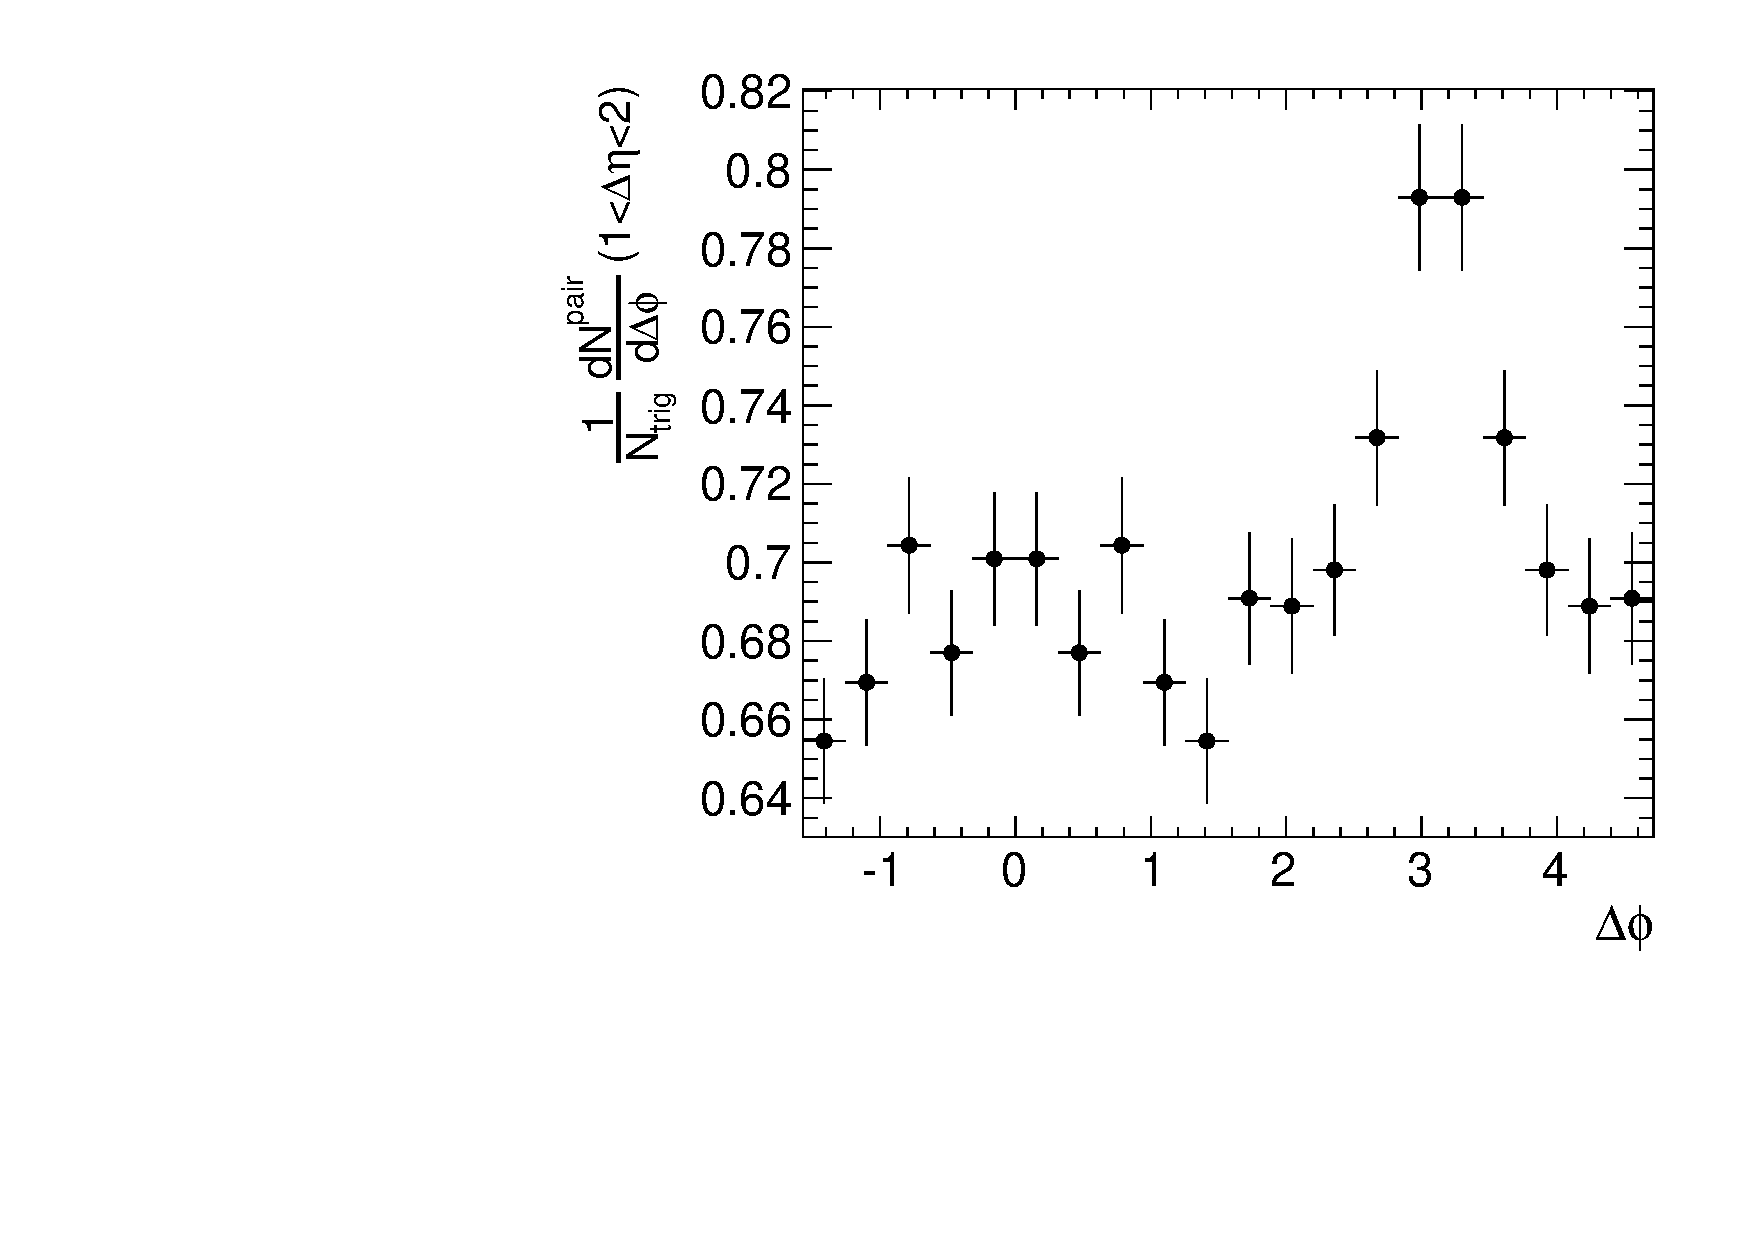
\includegraphics[width=.45\textwidth]{figures/canvasProjection_isBelle1_mult50_eta12.pdf}
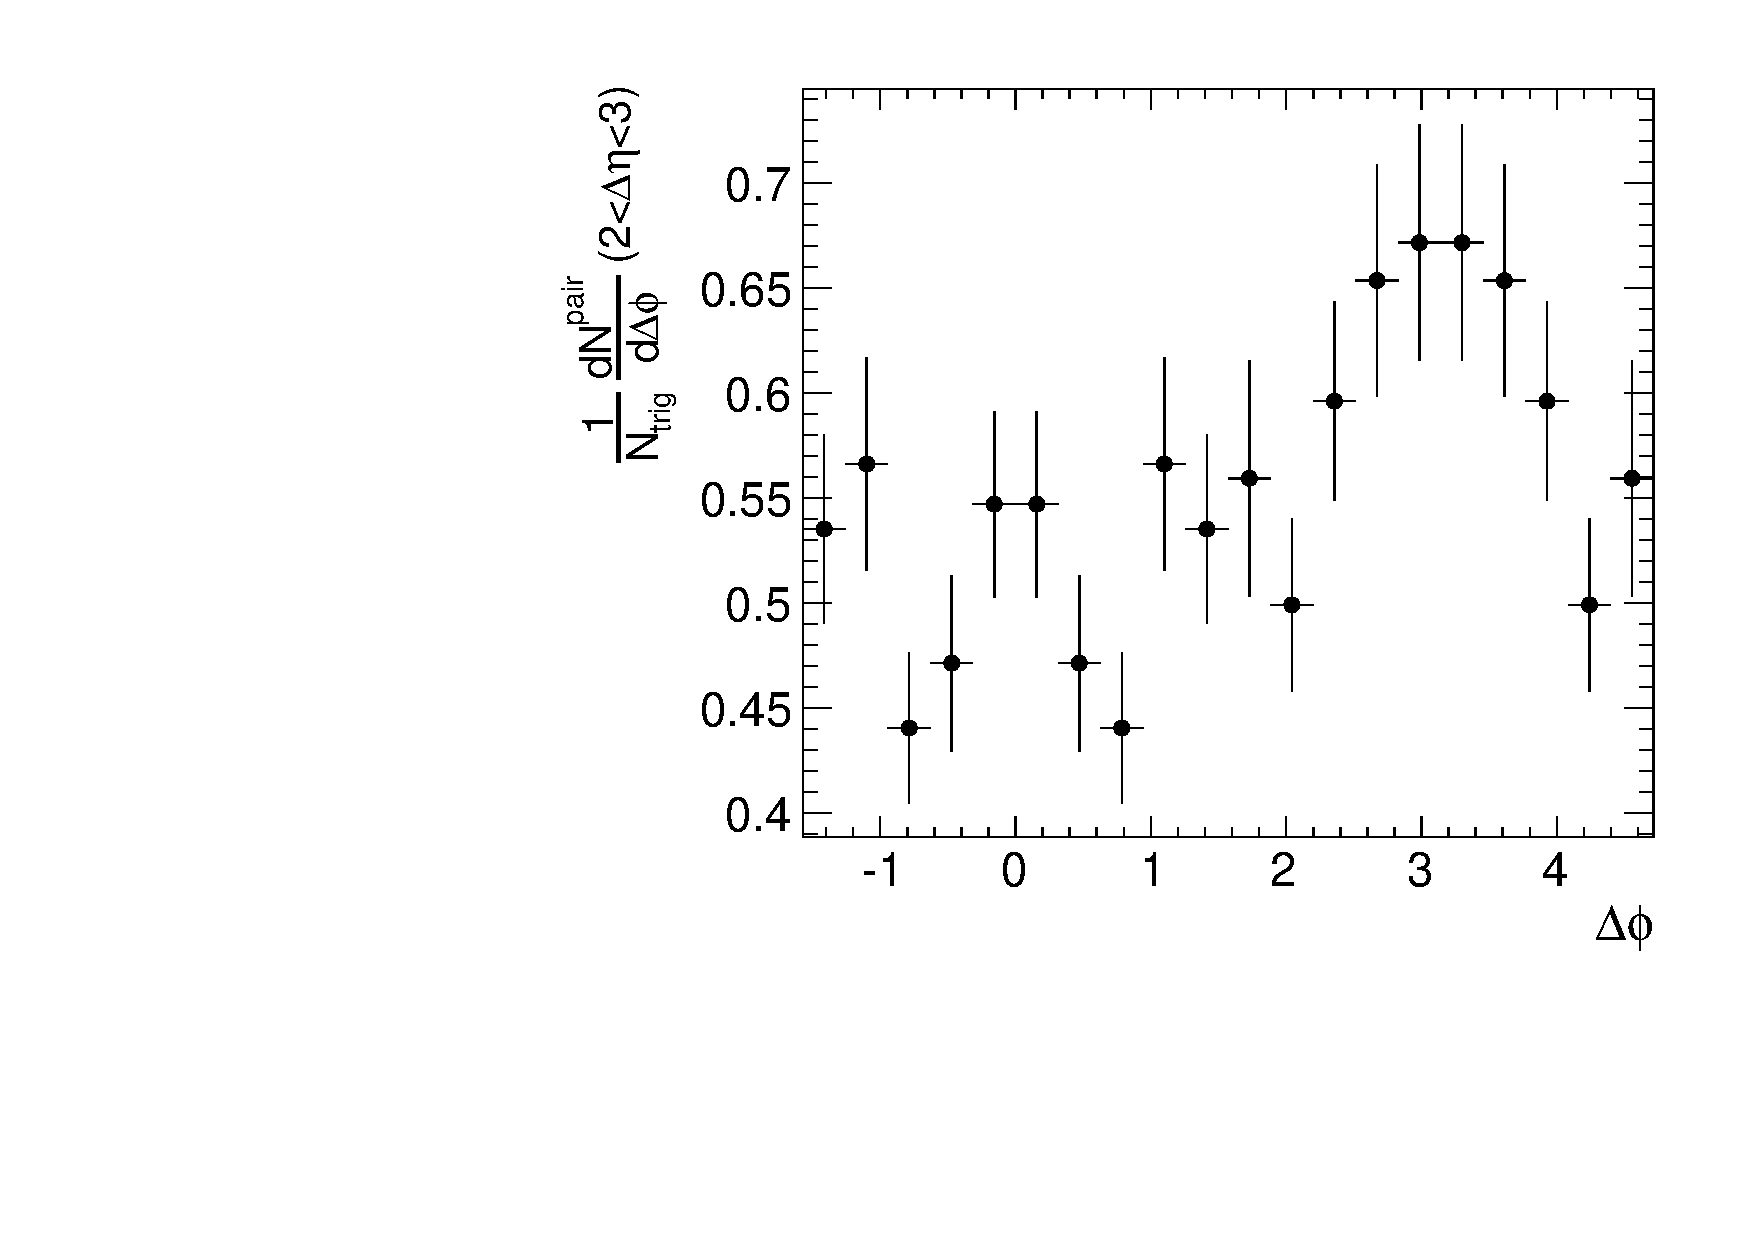
\includegraphics[width=.45\textwidth]{figures/canvasProjection_isBelle1_mult50_eta23.pdf}
\caption{$\rm \Delta R$ ($\rm \Delta\phi$) for events with total multiplicity N$>=$ 50. }
\label{fig:ProjectionMult50} 
\end{center}
\end{figure}
